\section*{Random-Sampling des NFW Profils}

Beim Random-Sampling wird eine zufällige Koordinate generiert und dessen
Abstand zum Mittelpunkt der Galaxie \( r \) berechnet.
Diesen Wert \( r \) setzt man in das NFW-Profil ein, um eine Wahrscheinlichkeit
\( \phi = \rho(r) \) zu berechnen, mit der der Stern generiert wird.
Es wird ein zufälliger Wert \( s \) im Intervall \( [\rho_{min};~\rho_{max}] \)
generiert.
Gilt \( s < r \), dann werden die Koordinaten des Sterns beibehalten,
ansonsten werden neue Koordinaten generiert und der Prozess wird wiederholt.

\begin{center}\vspace{-1cm}
\begin{equation} \label{eq:NFW_profile}
  \rho_{NFW}(r) = \frac{ 1 }{ \sqrt{ 2 \pi } \cdot \sigma } \cdot
  \exp \left( \frac{ -\phi(r) }{ \sigma^{ 2 } } \right)
\end{equation}

\begin{equation}
  \phi(r) = \frac{ 4\pi \cdot G \cdot f_{0} \cdot R_{s}^3 }{ r } \cdot
  ln{ \left( 1 + \frac{ r }{ R_{s} } \right) }
\end{equation}
\end{center}%\vspace{0.5cm}
%
\begin{center}\vspace{-0.5cm}
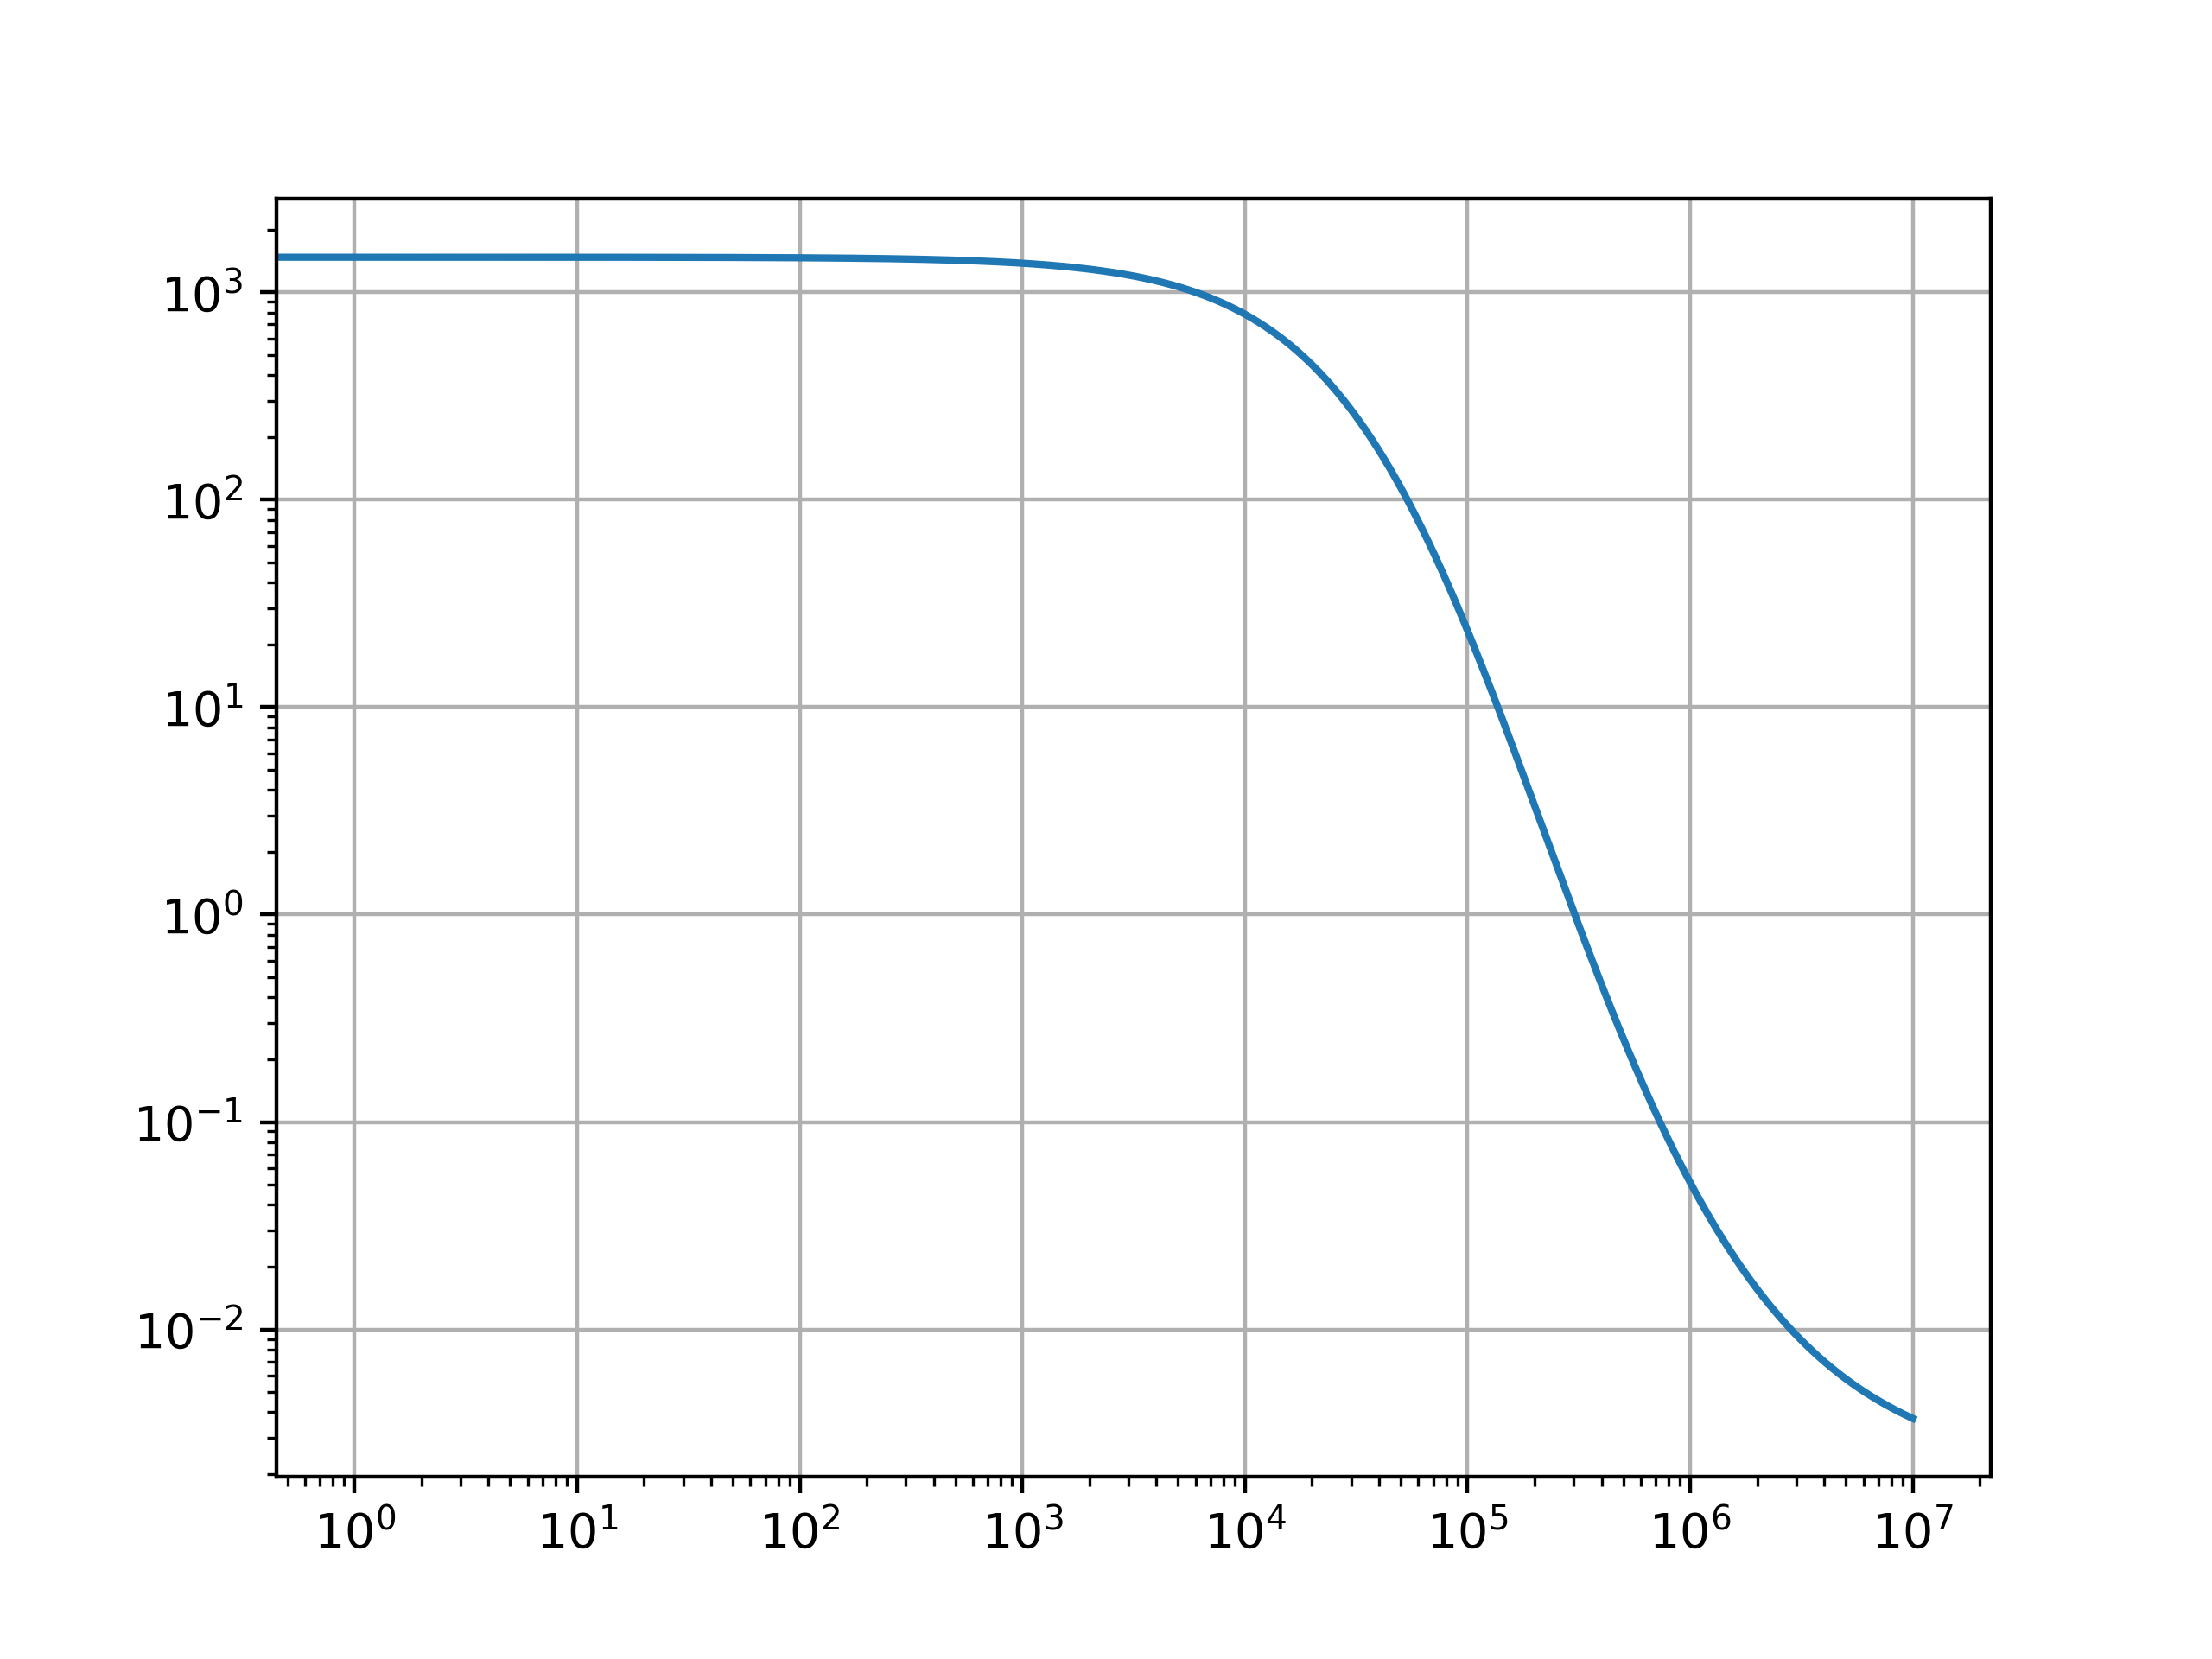
\includegraphics[width=0.8\linewidth]{figs/1e6_6}
\caption{Der entsprechende Funktionsgraph zum NFW-Profil}
\label{fig:lookup_NFW}
\end{center}\vspace{-1cm}
